\documentclass[twoside]{book}

% Packages required by doxygen
\usepackage{fixltx2e}
\usepackage{calc}
\usepackage{doxygen}
\usepackage{graphicx}
\usepackage[utf8]{inputenc}
\usepackage{makeidx}
\usepackage{multicol}
\usepackage{multirow}
\PassOptionsToPackage{warn}{textcomp}
\usepackage{textcomp}
\usepackage[nointegrals]{wasysym}
\usepackage[table]{xcolor}

% Font selection
\usepackage[T1]{fontenc}
\usepackage{mathptmx}
\usepackage[scaled=.90]{helvet}
\usepackage{courier}
\usepackage{amssymb}
\usepackage{sectsty}
\renewcommand{\familydefault}{\sfdefault}
\allsectionsfont{%
  \fontseries{bc}\selectfont%
  \color{darkgray}%
}
\renewcommand{\DoxyLabelFont}{%
  \fontseries{bc}\selectfont%
  \color{darkgray}%
}
\newcommand{\+}{\discretionary{\mbox{\scriptsize$\hookleftarrow$}}{}{}}

% Page & text layout
\usepackage{geometry}
\geometry{%
  a4paper,%
  top=2.5cm,%
  bottom=2.5cm,%
  left=2.5cm,%
  right=2.5cm%
}
\tolerance=750
\hfuzz=15pt
\hbadness=750
\setlength{\emergencystretch}{15pt}
\setlength{\parindent}{0cm}
\setlength{\parskip}{0.2cm}
\makeatletter
\renewcommand{\paragraph}{%
  \@startsection{paragraph}{4}{0ex}{-1.0ex}{1.0ex}{%
    \normalfont\normalsize\bfseries\SS@parafont%
  }%
}
\renewcommand{\subparagraph}{%
  \@startsection{subparagraph}{5}{0ex}{-1.0ex}{1.0ex}{%
    \normalfont\normalsize\bfseries\SS@subparafont%
  }%
}
\makeatother

% Headers & footers
\usepackage{fancyhdr}
\pagestyle{fancyplain}
\fancyhead[LE]{\fancyplain{}{\bfseries\thepage}}
\fancyhead[CE]{\fancyplain{}{}}
\fancyhead[RE]{\fancyplain{}{\bfseries\leftmark}}
\fancyhead[LO]{\fancyplain{}{\bfseries\rightmark}}
\fancyhead[CO]{\fancyplain{}{}}
\fancyhead[RO]{\fancyplain{}{\bfseries\thepage}}
\fancyfoot[LE]{\fancyplain{}{}}
\fancyfoot[CE]{\fancyplain{}{}}
\fancyfoot[RE]{\fancyplain{}{\bfseries\scriptsize Generated on Wed Mar 30 2016 11\+:54\+:27 for My Project by Doxygen }}
\fancyfoot[LO]{\fancyplain{}{\bfseries\scriptsize Generated on Wed Mar 30 2016 11\+:54\+:27 for My Project by Doxygen }}
\fancyfoot[CO]{\fancyplain{}{}}
\fancyfoot[RO]{\fancyplain{}{}}
\renewcommand{\footrulewidth}{0.4pt}
\renewcommand{\chaptermark}[1]{%
  \markboth{#1}{}%
}
\renewcommand{\sectionmark}[1]{%
  \markright{\thesection\ #1}%
}

% Indices & bibliography
\usepackage{natbib}
\usepackage[titles]{tocloft}
\setcounter{tocdepth}{3}
\setcounter{secnumdepth}{5}
\makeindex

% Hyperlinks (required, but should be loaded last)
\usepackage{ifpdf}
\ifpdf
  \usepackage[pdftex,pagebackref=true]{hyperref}
\else
  \usepackage[ps2pdf,pagebackref=true]{hyperref}
\fi
\hypersetup{%
  colorlinks=true,%
  linkcolor=blue,%
  citecolor=blue,%
  unicode%
}

% Custom commands
\newcommand{\clearemptydoublepage}{%
  \newpage{\pagestyle{empty}\cleardoublepage}%
}


%===== C O N T E N T S =====

\begin{document}

% Titlepage & ToC
\hypersetup{pageanchor=false,
             bookmarks=true,
             bookmarksnumbered=true,
             pdfencoding=unicode
            }
\pagenumbering{roman}
\begin{titlepage}
\vspace*{7cm}
\begin{center}%
{\Large My Project }\\
\vspace*{1cm}
{\large Generated by Doxygen 1.8.8}\\
\vspace*{0.5cm}
{\small Wed Mar 30 2016 11:54:27}\\
\end{center}
\end{titlepage}
\clearemptydoublepage
\tableofcontents
\clearemptydoublepage
\pagenumbering{arabic}
\hypersetup{pageanchor=true}

%--- Begin generated contents ---
\chapter{Namespace Index}
\section{Namespace List}
Here is a list of all namespaces with brief descriptions\+:\begin{DoxyCompactList}
\item\contentsline{section}{\hyperlink{namespacevaso}{vaso} \\*Function()s related to the program's threaded processing of audio data }{\pageref{namespacevaso}}{}
\end{DoxyCompactList}

\chapter{Class Index}
\section{Class List}
Here are the classes, structs, unions and interfaces with brief descriptions\+:\begin{DoxyCompactList}
\item\contentsline{section}{\hyperlink{structDataParams}{Data\+Params} }{\pageref{structDataParams}}{}
\item\contentsline{section}{\hyperlink{structMaximum}{Maximum} }{\pageref{structMaximum}}{}
\end{DoxyCompactList}

\chapter{File Index}
\section{File List}
Here is a list of all files with brief descriptions\+:\begin{DoxyCompactList}
\item\contentsline{section}{\hyperlink{makefile}{makefile} \\*Contains recipes for building the test applications, the main application, and the documentation }{\pageref{makefile}}{}
\item\contentsline{section}{etc/\hyperlink{doxygen_8config}{doxygen.\+config} \\*Contains Doxygen configuration settings }{\pageref{doxygen_8config}}{}
\item\contentsline{section}{src/\hyperlink{definitions_8hpp}{definitions.\+hpp} \\*Contains declarations of system-\/independant (universal size) integers and float types, shortened type names for some commonly used types, and enumerations }{\pageref{definitions_8hpp}}{}
\item\contentsline{section}{src/\hyperlink{fileio_8hpp}{fileio.\+hpp} \\*Functions related to the file I/\+O use in this program }{\pageref{fileio_8hpp}}{}
\item\contentsline{section}{src/\hyperlink{fileio__test_8cpp}{fileio\+\_\+test.\+cpp} \\*Contains program that tests the functions in \hyperlink{fileio_8hpp}{fileio.\+hpp} }{\pageref{fileio__test_8cpp}}{}
\item\contentsline{section}{src/\hyperlink{main_8cpp}{main.\+cpp} \\*Contains the main program }{\pageref{main_8cpp}}{}
\item\contentsline{section}{src/\hyperlink{patient__name__test_8cpp}{patient\+\_\+name\+\_\+test.\+cpp} \\*Contains a program to test the \hyperlink{namespaceavda_ae20728e7e8ae50bf2f74849e538841ea}{Patient\+Name()} function }{\pageref{patient__name__test_8cpp}}{}
\item\contentsline{section}{src/\hyperlink{process_8hpp}{process.\+hpp} \\*Contains functions related to the program's threaded processing of audio data }{\pageref{process_8hpp}}{}
\item\contentsline{section}{src/\hyperlink{process__test_8cpp}{process\+\_\+test.\+cpp} \\*Contains a program to test the \hyperlink{namespaceavda_a5196cce27286d08ca144a460caee7839}{process()} function }{\pageref{process__test_8cpp}}{}
\item\contentsline{section}{src/\hyperlink{read__params__test_8cpp}{read\+\_\+params\+\_\+test.\+cpp} \\*Contains a program test the \hyperlink{namespaceavda_ae20728e7e8ae50bf2f74849e538841ea}{Patient\+Name()} function }{\pageref{read__params__test_8cpp}}{}
\item\contentsline{section}{src/\hyperlink{sigmath_8hpp}{sigmath.\+hpp} \\*Functions necessary to perform the mathematical operations required by this program }{\pageref{sigmath_8hpp}}{}
\item\contentsline{section}{src/\hyperlink{sound_8hpp}{sound.\+hpp} \\*Function(s) relating to sound }{\pageref{sound_8hpp}}{}
\item\contentsline{section}{src/\hyperlink{stdin__clear__test_8cpp}{stdin\+\_\+clear\+\_\+test.\+cpp} \\*Contains a program to test clearing the stdin buffer }{\pageref{stdin__clear__test_8cpp}}{}
\end{DoxyCompactList}

\chapter{Namespace Documentation}
\hypertarget{namespacevaso}{\section{vaso Namespace Reference}
\label{namespacevaso}\index{vaso@{vaso}}
}


contains functions related to the file I/\+O use in this program  


\subsection*{Enumerations}
\begin{DoxyCompactItemize}
\item 
enum \hyperlink{namespacevaso_a77c5d9704657d49d456f691ddd8abf7c}{Side} \{ \hyperlink{namespacevaso_a77c5d9704657d49d456f691ddd8abf7ca945d5e233cf7d6240f6b783b36a374ff}{Side\+::\+Left}, 
\hyperlink{namespacevaso_a77c5d9704657d49d456f691ddd8abf7ca92b09c7c48c520c3c55e497875da437c}{Side\+::\+Right}
 \}
\end{DoxyCompactItemize}
\subsection*{Functions}
\begin{DoxyCompactItemize}
\item 
std\+::string \hyperlink{namespacevaso_abab641a332f2e834dfcdf294c0429426}{Current\+Data\+Name} ()
\item 
std\+::string \hyperlink{namespacevaso_af8f45524d4770053c2b812ce33a7095f}{Initial\+Data\+Name} (auto dir)
\item 
std\+::string \hyperlink{namespacevaso_a21e264fa912f7ca3f50e7e412ba1582e}{Patient\+Name} ()
\item 
\hyperlink{structDataParams}{Data\+Params} \hyperlink{namespacevaso_a6f1a23c617aae2e2c4af5e8016b4d03e}{Read\+Params} (auto filename)
\item 
std\+::string \hyperlink{namespacevaso_ad8543c0caabf3836b4a93a78e0d487d1}{Write\+Params} (\hyperlink{structDataParams}{Data\+Params} params, auto filename)
\item 
void \hyperlink{namespacevaso_a9d0e5d69685ee494d286db6ece005156}{average} (\hyperlink{definitions_8hpp_aacdc525d6f7bddb3ae95d5c311bd06a1}{float32} $\ast$data, \hyperlink{definitions_8hpp_aacdc525d6f7bddb3ae95d5c311bd06a1}{float32} $\ast$avg, \hyperlink{definitions_8hpp_adde6aaee8457bee49c2a92621fe22b79}{uint8} count, \hyperlink{definitions_8hpp_a1134b580f8da4de94ca6b1de4d37975e}{uint32} size)
\item 
void \hyperlink{namespacevaso_a7d108bce812e906d8b1810815774c7ea}{diff} (\hyperlink{definitions_8hpp_aacdc525d6f7bddb3ae95d5c311bd06a1}{float32} $\ast$data, \hyperlink{definitions_8hpp_a1134b580f8da4de94ca6b1de4d37975e}{uint32} size)
\item 
void \hyperlink{namespacevaso_af74f08a8afd7967b6c2b3c2b0e5fb1e9}{fft} (\hyperlink{definitions_8hpp_a960be6b6614c08090c16574dba10a421}{cfloat32} $\ast$data, \hyperlink{definitions_8hpp_a1134b580f8da4de94ca6b1de4d37975e}{uint32} size)
\item 
void \hyperlink{namespacevaso_a5d355b5c326a852e2ce95c258450898c}{mag} (\hyperlink{definitions_8hpp_a960be6b6614c08090c16574dba10a421}{cfloat32} $\ast$orig, \hyperlink{definitions_8hpp_aacdc525d6f7bddb3ae95d5c311bd06a1}{float32} $\ast$newmags, \hyperlink{definitions_8hpp_a1134b580f8da4de94ca6b1de4d37975e}{uint32} size)
\item 
void \hyperlink{namespacevaso_a649803d9dd74002f7975dba6b48b56ce}{max} (\hyperlink{definitions_8hpp_aacdc525d6f7bddb3ae95d5c311bd06a1}{float32} $\ast$data, \hyperlink{definitions_8hpp_a1134b580f8da4de94ca6b1de4d37975e}{uint32} size)
\item 
void \hyperlink{namespacevaso_a5b7fc1a58199e2cac989f417a9faa1ce}{smooth} (\hyperlink{definitions_8hpp_aacdc525d6f7bddb3ae95d5c311bd06a1}{float32} $\ast$data, \hyperlink{definitions_8hpp_a1134b580f8da4de94ca6b1de4d37975e}{uint32} size, \hyperlink{definitions_8hpp_a05f6b0ae8f6a6e135b0e290c25fe0e4e}{uint16} order)
\item 
void \hyperlink{namespacevaso_a7da499b9b1b5a492bea8ab8681e57c22}{play} (auto filename)
\item 
void $\ast$ \hyperlink{namespacevaso_acd767ffd09e8d7323a0275e8f88a6de2}{process} (void $\ast$procdata)
\item 
void \hyperlink{namespacevaso_aec526a2735f71ef68cea3e00ae943edf}{Start\+Processing} (\hyperlink{structProcData}{Proc\+Data} procdata)
\item 
void $\ast$ \hyperlink{namespacevaso_ae553d67666b43a570bbb1753b2a624d2}{processing} (void $\ast$procdata)
\end{DoxyCompactItemize}
\subsection*{Variables}
\begin{DoxyCompactItemize}
\item 
const std\+::string \hyperlink{namespacevaso_a0f49c8240a13e7d853912ad78d5f53c9}{P\+A\+T\+I\+E\+N\+T\+\_\+\+P\+A\+T\+H} = \char`\"{}/home/pi/patients/\char`\"{}
\end{DoxyCompactItemize}


\subsection{Detailed Description}
contains functions related to the file I/\+O use in this program 

contains functions related to the program's threaded processing of audio data

contains the function(s) relating to sound

contains the functions necessary to perform the mathematical operations required by this program

This namespace contains all code related to this project.

\begin{DoxyAuthor}{Author}
Samuel Andrew Wisner, \href{mailto:awisner94@gmail.com}{\tt awisner94@gmail.\+com}

Samuel Andrew Wisner, \href{mailto:awisner94@gmail.com}{\tt awisner94@gmail.\+com} 

Nicholas K. Nolan

Samuel Andrew Wisner, \href{mailto:awisne94@gmail.com}{\tt awisne94@gmail.\+com} 
\end{DoxyAuthor}


\subsection{Enumeration Type Documentation}
\hypertarget{namespacevaso_a77c5d9704657d49d456f691ddd8abf7c}{\index{vaso@{vaso}!Side@{Side}}
\index{Side@{Side}!vaso@{vaso}}
\subsubsection[{Side}]{\setlength{\rightskip}{0pt plus 5cm}enum {\bf vaso\+::\+Side}\hspace{0.3cm}{\ttfamily [strong]}}}\label{namespacevaso_a77c5d9704657d49d456f691ddd8abf7c}
The side of the head to which a recording pertains. \begin{Desc}
\item[Enumerator]\par
\begin{description}
\index{Left@{Left}!vaso@{vaso}}\index{vaso@{vaso}!Left@{Left}}\item[{\em 
\hypertarget{namespacevaso_a77c5d9704657d49d456f691ddd8abf7ca945d5e233cf7d6240f6b783b36a374ff}{Left}\label{namespacevaso_a77c5d9704657d49d456f691ddd8abf7ca945d5e233cf7d6240f6b783b36a374ff}
}]\index{Right@{Right}!vaso@{vaso}}\index{vaso@{vaso}!Right@{Right}}\item[{\em 
\hypertarget{namespacevaso_a77c5d9704657d49d456f691ddd8abf7ca92b09c7c48c520c3c55e497875da437c}{Right}\label{namespacevaso_a77c5d9704657d49d456f691ddd8abf7ca92b09c7c48c520c3c55e497875da437c}
}]\end{description}
\end{Desc}


Definition at line 58 of file definitions.\+hpp.



\subsection{Function Documentation}
\hypertarget{namespacevaso_a9d0e5d69685ee494d286db6ece005156}{\index{vaso@{vaso}!average@{average}}
\index{average@{average}!vaso@{vaso}}
\subsubsection[{average}]{\setlength{\rightskip}{0pt plus 5cm}void vaso\+::average (
\begin{DoxyParamCaption}
\item[{{\bf float32} $\ast$}]{data, }
\item[{{\bf float32} $\ast$}]{avg, }
\item[{{\bf uint8}}]{count, }
\item[{{\bf uint32}}]{size}
\end{DoxyParamCaption}
)}}\label{namespacevaso_a9d0e5d69685ee494d286db6ece005156}
Element-\/wise averaging along the first dimension of a two-\/dimensional array.


\begin{DoxyParams}{Parameters}
{\em data} & the two-\/dimensional array containing \mbox{[}count\mbox{]} number of arrays in the first dimension and \mbox{[}size\mbox{]} number of each elements in the second dimension\\
\hline
{\em avg} & the array of size \mbox{[}size\mbox{]} containing the averaged values of each element\\
\hline
{\em count} & the number of arrays in the first dimension of data and will likely be a constant value of 3 in this program\\
\hline
{\em size} & the number of elements in the second dimension of data \\
\hline
\end{DoxyParams}


Definition at line 94 of file sigmath.\+hpp.

\hypertarget{namespacevaso_abab641a332f2e834dfcdf294c0429426}{\index{vaso@{vaso}!Current\+Data\+Name@{Current\+Data\+Name}}
\index{Current\+Data\+Name@{Current\+Data\+Name}!vaso@{vaso}}
\subsubsection[{Current\+Data\+Name}]{\setlength{\rightskip}{0pt plus 5cm}std\+::string vaso\+::\+Current\+Data\+Name (
\begin{DoxyParamCaption}
{}
\end{DoxyParamCaption}
)}}\label{namespacevaso_abab641a332f2e834dfcdf294c0429426}
Gets a data-\/based name to which the file(s) created in a session to be saved.

\begin{DoxyReturn}{Returns}
a partial (?) filename for the current session 
\end{DoxyReturn}


Definition at line 26 of file fileio.\+hpp.

\hypertarget{namespacevaso_a7d108bce812e906d8b1810815774c7ea}{\index{vaso@{vaso}!diff@{diff}}
\index{diff@{diff}!vaso@{vaso}}
\subsubsection[{diff}]{\setlength{\rightskip}{0pt plus 5cm}void vaso\+::diff (
\begin{DoxyParamCaption}
\item[{{\bf float32} $\ast$}]{data, }
\item[{{\bf uint32}}]{size}
\end{DoxyParamCaption}
)}}\label{namespacevaso_a7d108bce812e906d8b1810815774c7ea}
Computes the left-\/handed first derivative of a discrete signal. The first element will be 0.


\begin{DoxyParams}{Parameters}
{\em data} & an array containing the discrete signal data\\
\hline
{\em size} & the number of elements in data \\
\hline
\end{DoxyParams}


Definition at line 98 of file sigmath.\+hpp.

\hypertarget{namespacevaso_af74f08a8afd7967b6c2b3c2b0e5fb1e9}{\index{vaso@{vaso}!fft@{fft}}
\index{fft@{fft}!vaso@{vaso}}
\subsubsection[{fft}]{\setlength{\rightskip}{0pt plus 5cm}void vaso\+::fft (
\begin{DoxyParamCaption}
\item[{{\bf cfloat32} $\ast$}]{data, }
\item[{{\bf uint32}}]{size}
\end{DoxyParamCaption}
)}}\label{namespacevaso_af74f08a8afd7967b6c2b3c2b0e5fb1e9}
Replaces the values of an array of cfloat32's with the array's D\+F\+T using a decimation-\/in-\/frequency algorithm.

This code is based on code from \href{http://rosettacode.org/wiki/Fast_Fourier_transform#C.2B.2B}{\tt http\+://rosettacode.\+org/wiki/\+Fast\+\_\+\+Fourier\+\_\+transform\#\+C.\+2\+B.\+2\+B}.


\begin{DoxyParams}{Parameters}
{\em data} & the array whose values should be replaced with its D\+F\+T\\
\hline
{\em size} & the number of elements in the data array \\
\hline
\end{DoxyParams}


Definition at line 102 of file sigmath.\+hpp.

\hypertarget{namespacevaso_af8f45524d4770053c2b812ce33a7095f}{\index{vaso@{vaso}!Initial\+Data\+Name@{Initial\+Data\+Name}}
\index{Initial\+Data\+Name@{Initial\+Data\+Name}!vaso@{vaso}}
\subsubsection[{Initial\+Data\+Name}]{\setlength{\rightskip}{0pt plus 5cm}std\+::string vaso\+::\+Initial\+Data\+Name (
\begin{DoxyParamCaption}
\item[{auto}]{dir}
\end{DoxyParamCaption}
)}}\label{namespacevaso_af8f45524d4770053c2b812ce33a7095f}
Finds the filename of the oldest (i.\+e., baseline) data is saved.


\begin{DoxyParams}{Parameters}
{\em dir} & the directory which contains all patient data\\
\hline
\end{DoxyParams}
\begin{DoxyReturn}{Returns}
the base (?) filename to which all baseline data was saved 
\end{DoxyReturn}


Definition at line 37 of file fileio.\+hpp.

\hypertarget{namespacevaso_a5d355b5c326a852e2ce95c258450898c}{\index{vaso@{vaso}!mag@{mag}}
\index{mag@{mag}!vaso@{vaso}}
\subsubsection[{mag}]{\setlength{\rightskip}{0pt plus 5cm}void vaso\+::mag (
\begin{DoxyParamCaption}
\item[{{\bf cfloat32} $\ast$}]{orig, }
\item[{{\bf float32} $\ast$}]{newmags, }
\item[{{\bf uint32}}]{size}
\end{DoxyParamCaption}
)}}\label{namespacevaso_a5d355b5c326a852e2ce95c258450898c}
Computes the magitude of an array of complex numbers.


\begin{DoxyParams}{Parameters}
{\em orig} & the array of complex numbers\\
\hline
{\em newmags} & an array to which the magitudes are to be written\\
\hline
{\em size} & the number of elements in orig and newmags \\
\hline
\end{DoxyParams}


Definition at line 150 of file sigmath.\+hpp.

\hypertarget{namespacevaso_a649803d9dd74002f7975dba6b48b56ce}{\index{vaso@{vaso}!max@{max}}
\index{max@{max}!vaso@{vaso}}
\subsubsection[{max}]{\setlength{\rightskip}{0pt plus 5cm}void vaso\+::max (
\begin{DoxyParamCaption}
\item[{{\bf float32} $\ast$}]{data, }
\item[{{\bf uint32}}]{size}
\end{DoxyParamCaption}
)}}\label{namespacevaso_a649803d9dd74002f7975dba6b48b56ce}
Finds the maximum value in an array.


\begin{DoxyParams}{Parameters}
{\em data} & the array whose maximum value is to be found\\
\hline
{\em uint32} & size the number of elements in the data array \\
\hline
\end{DoxyParams}


Definition at line 154 of file sigmath.\+hpp.

\hypertarget{namespacevaso_a21e264fa912f7ca3f50e7e412ba1582e}{\index{vaso@{vaso}!Patient\+Name@{Patient\+Name}}
\index{Patient\+Name@{Patient\+Name}!vaso@{vaso}}
\subsubsection[{Patient\+Name}]{\setlength{\rightskip}{0pt plus 5cm}std\+::string vaso\+::\+Patient\+Name (
\begin{DoxyParamCaption}
{}
\end{DoxyParamCaption}
)}}\label{namespacevaso_a21e264fa912f7ca3f50e7e412ba1582e}
Prompts a user to enter a first, middle, and last name for a patients and creates a directory (if necessary) in which all of a patient's data can be saved.

Must warn a user if the patient folder does not already exist in order to prevent missaving data.

\begin{DoxyReturn}{Returns}
the directory under which all patient data is saved 
\end{DoxyReturn}


Definition at line 51 of file fileio.\+hpp.

\hypertarget{namespacevaso_a7da499b9b1b5a492bea8ab8681e57c22}{\index{vaso@{vaso}!play@{play}}
\index{play@{play}!vaso@{vaso}}
\subsubsection[{play}]{\setlength{\rightskip}{0pt plus 5cm}void vaso\+::play (
\begin{DoxyParamCaption}
\item[{auto}]{filename}
\end{DoxyParamCaption}
)}}\label{namespacevaso_a7da499b9b1b5a492bea8ab8681e57c22}
Plays a W\+A\+V\+E file in a loop in a non-\/blocking manner.


\begin{DoxyParams}{Parameters}
{\em filename} & the absolute or relative path to the W\+A\+V\+E file \\
\hline
\end{DoxyParams}


Definition at line 19 of file sound.\+hpp.

\hypertarget{namespacevaso_acd767ffd09e8d7323a0275e8f88a6de2}{\index{vaso@{vaso}!process@{process}}
\index{process@{process}!vaso@{vaso}}
\subsubsection[{process}]{\setlength{\rightskip}{0pt plus 5cm}void$\ast$ vaso\+::process (
\begin{DoxyParamCaption}
\item[{void $\ast$}]{procdata}
\end{DoxyParamCaption}
)}}\label{namespacevaso_acd767ffd09e8d7323a0275e8f88a6de2}
Computes recording parameters in a separate thread in a thread-\/safe manner. A\+Utomatically waits for each recording to finish before processing it. This file is meant to be called O\+N\+L\+Y from the Start\+Processing function.


\begin{DoxyParams}{Parameters}
{\em procdata} & a struct containing the values necessary to processing the audio\\
\hline
\end{DoxyParams}
\begin{DoxyReturn}{Returns}
a (void) pointer to a \hyperlink{structDataParams}{Data\+Params} struct containing the computed parameters for a patient 
\end{DoxyReturn}
\hypertarget{namespacevaso_ae553d67666b43a570bbb1753b2a624d2}{\index{vaso@{vaso}!processing@{processing}}
\index{processing@{processing}!vaso@{vaso}}
\subsubsection[{processing}]{\setlength{\rightskip}{0pt plus 5cm}void$\ast$ vaso\+::processing (
\begin{DoxyParamCaption}
\item[{void $\ast$}]{procdata}
\end{DoxyParamCaption}
)}}\label{namespacevaso_ae553d67666b43a570bbb1753b2a624d2}


Definition at line 42 of file threadproc.\+hpp.

\hypertarget{namespacevaso_a6f1a23c617aae2e2c4af5e8016b4d03e}{\index{vaso@{vaso}!Read\+Params@{Read\+Params}}
\index{Read\+Params@{Read\+Params}!vaso@{vaso}}
\subsubsection[{Read\+Params}]{\setlength{\rightskip}{0pt plus 5cm}{\bf Data\+Params} vaso\+::\+Read\+Params (
\begin{DoxyParamCaption}
\item[{auto}]{filename}
\end{DoxyParamCaption}
)}}\label{namespacevaso_a6f1a23c617aae2e2c4af5e8016b4d03e}
Reads the previously computated parameters found in the specified file.


\begin{DoxyParams}{Parameters}
{\em filename} & the absolute or relative path to the file containing the patient data to read\\
\hline
\end{DoxyParams}
\begin{DoxyReturn}{Returns}
the patient parameters read 
\end{DoxyReturn}


Definition at line 64 of file fileio.\+hpp.

\hypertarget{namespacevaso_a5b7fc1a58199e2cac989f417a9faa1ce}{\index{vaso@{vaso}!smooth@{smooth}}
\index{smooth@{smooth}!vaso@{vaso}}
\subsubsection[{smooth}]{\setlength{\rightskip}{0pt plus 5cm}void vaso\+::smooth (
\begin{DoxyParamCaption}
\item[{{\bf float32} $\ast$}]{data, }
\item[{{\bf uint32}}]{size, }
\item[{{\bf uint16}}]{order}
\end{DoxyParamCaption}
)}}\label{namespacevaso_a5b7fc1a58199e2cac989f417a9faa1ce}
Applies an nth-\/order moving-\/average filter to a discrete signal.


\begin{DoxyParams}{Parameters}
{\em data} & the array containing the signal to which the filter should be applied\\
\hline
{\em size} & the number of elements in the data array\\
\hline
{\em order} & the order of the filter \\
\hline
\end{DoxyParams}


Definition at line 158 of file sigmath.\+hpp.

\hypertarget{namespacevaso_aec526a2735f71ef68cea3e00ae943edf}{\index{vaso@{vaso}!Start\+Processing@{Start\+Processing}}
\index{Start\+Processing@{Start\+Processing}!vaso@{vaso}}
\subsubsection[{Start\+Processing}]{\setlength{\rightskip}{0pt plus 5cm}void vaso\+::\+Start\+Processing (
\begin{DoxyParamCaption}
\item[{{\bf Proc\+Data}}]{procdata}
\end{DoxyParamCaption}
)}}\label{namespacevaso_aec526a2735f71ef68cea3e00ae943edf}
Begins processing the recorded data. Should be called before or immediately after the first recording.


\begin{DoxyParams}{Parameters}
{\em proxdata} & a struct containing the values necessary to processing the audio \\
\hline
\end{DoxyParams}


Definition at line 46 of file threadproc.\+hpp.

\hypertarget{namespacevaso_ad8543c0caabf3836b4a93a78e0d487d1}{\index{vaso@{vaso}!Write\+Params@{Write\+Params}}
\index{Write\+Params@{Write\+Params}!vaso@{vaso}}
\subsubsection[{Write\+Params}]{\setlength{\rightskip}{0pt plus 5cm}std\+::string vaso\+::\+Write\+Params (
\begin{DoxyParamCaption}
\item[{{\bf Data\+Params}}]{params, }
\item[{auto}]{filename}
\end{DoxyParamCaption}
)}}\label{namespacevaso_ad8543c0caabf3836b4a93a78e0d487d1}
Writes the parameters to the specified file.


\begin{DoxyParams}{Parameters}
{\em params} & \\
\hline
\end{DoxyParams}


Definition at line 73 of file fileio.\+hpp.



\subsection{Variable Documentation}
\hypertarget{namespacevaso_a0f49c8240a13e7d853912ad78d5f53c9}{\index{vaso@{vaso}!P\+A\+T\+I\+E\+N\+T\+\_\+\+P\+A\+T\+H@{P\+A\+T\+I\+E\+N\+T\+\_\+\+P\+A\+T\+H}}
\index{P\+A\+T\+I\+E\+N\+T\+\_\+\+P\+A\+T\+H@{P\+A\+T\+I\+E\+N\+T\+\_\+\+P\+A\+T\+H}!vaso@{vaso}}
\subsubsection[{P\+A\+T\+I\+E\+N\+T\+\_\+\+P\+A\+T\+H}]{\setlength{\rightskip}{0pt plus 5cm}const std\+::string vaso\+::\+P\+A\+T\+I\+E\+N\+T\+\_\+\+P\+A\+T\+H = \char`\"{}/home/pi/patients/\char`\"{}}}\label{namespacevaso_a0f49c8240a13e7d853912ad78d5f53c9}
Absolute path to the folder containing the patients' data 

Definition at line 18 of file fileio.\+hpp.


\chapter{Class Documentation}
\hypertarget{structDataParams}{\section{Data\+Params Struct Reference}
\label{structDataParams}\index{Data\+Params@{Data\+Params}}
}


{\ttfamily \#include $<$definitions.\+hpp$>$}



\subsection{Detailed Description}
A structure containing the calculated results from processing the audio recordings. 

Definition at line 40 of file definitions.\+hpp.



The documentation for this struct was generated from the following file\+:\begin{DoxyCompactItemize}
\item 
src/\hyperlink{definitions_8hpp}{definitions.\+hpp}\end{DoxyCompactItemize}

\hypertarget{structProcData}{\section{Proc\+Data Struct Reference}
\label{structProcData}\index{Proc\+Data@{Proc\+Data}}
}


{\ttfamily \#include $<$definitions.\+hpp$>$}



\subsection{Detailed Description}


Definition at line 46 of file definitions.\+hpp.



The documentation for this struct was generated from the following file\+:\begin{DoxyCompactItemize}
\item 
src/\hyperlink{definitions_8hpp}{definitions.\+hpp}\end{DoxyCompactItemize}

\chapter{File Documentation}
\hypertarget{start}{\section{bin/start File Reference}
\label{start}\index{bin/start@{bin/start}}
}

\hypertarget{doxygen_8config}{\section{etc/doxygen.config File Reference}
\label{doxygen_8config}\index{etc/doxygen.\+config@{etc/doxygen.\+config}}
}

\hypertarget{makefile}{\section{makefile File Reference}
\label{makefile}\index{makefile@{makefile}}
}


Contains recipes for building the test applications, the main application, and the documentation.  




\subsection{Detailed Description}
Contains recipes for building the test applications, the main application, and the documentation. 

\begin{DoxyAuthor}{Author}
Samuel Andrew Wisner, \href{mailto:awisner94@gmail.com}{\tt awisner94@gmail.\+com} 
\end{DoxyAuthor}


Definition in file \hyperlink{makefile_source}{makefile}.


\hypertarget{definitions_8hpp}{\section{src/definitions.hpp File Reference}
\label{definitions_8hpp}\index{src/definitions.\+hpp@{src/definitions.\+hpp}}
}
{\ttfamily \#include $<$complex$>$}\\*
{\ttfamily \#include $<$map$>$}\\*
Include dependency graph for definitions.\+hpp\+:
\nopagebreak
\begin{figure}[H]
\begin{center}
\leavevmode
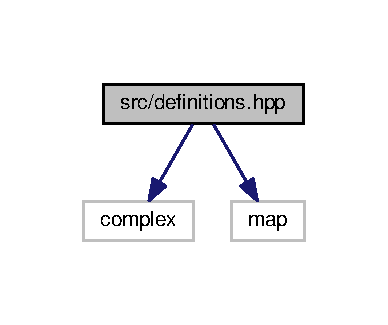
\includegraphics[width=186pt]{definitions_8hpp__incl}
\end{center}
\end{figure}
This graph shows which files directly or indirectly include this file\+:
\nopagebreak
\begin{figure}[H]
\begin{center}
\leavevmode
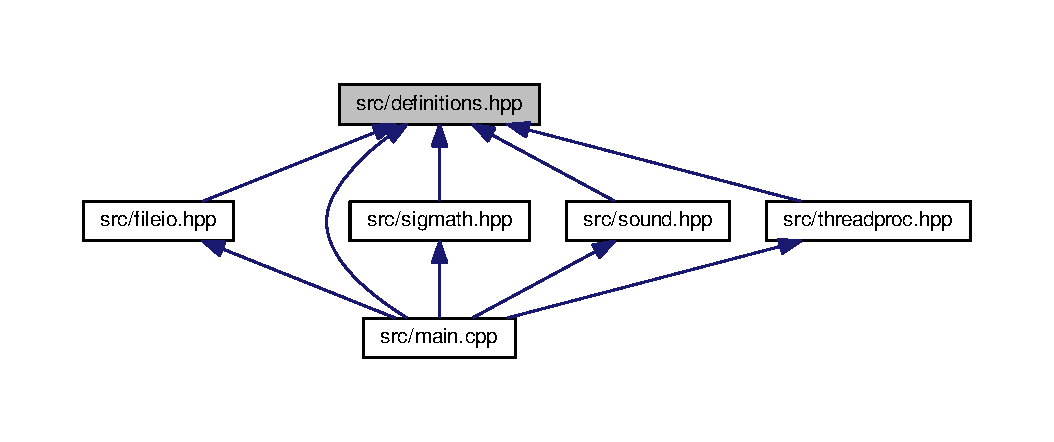
\includegraphics[width=350pt]{definitions_8hpp__dep__incl}
\end{center}
\end{figure}
\subsection*{Classes}
\begin{DoxyCompactItemize}
\item 
struct \hyperlink{structDataParams}{Data\+Params}
\item 
struct \hyperlink{structMaximum}{Maximum}
\item 
struct \hyperlink{structThreadParams}{Thread\+Params}
\end{DoxyCompactItemize}
\subsection*{Namespaces}
\begin{DoxyCompactItemize}
\item 
 \hyperlink{namespacevaso}{vaso}
\begin{DoxyCompactList}\small\item\em contains functions related to the file I/\+O use in this program \end{DoxyCompactList}\end{DoxyCompactItemize}
\subsection*{Macros}
\begin{DoxyCompactItemize}
\item 
\#define \hyperlink{definitions_8hpp_a8fe83ac76edc595f6b98cd4a4127aed5}{E\+R\+R\+O\+R}~-\/1
\begin{DoxyCompactList}\small\item\em Contains declarations of system-\/independant (universal size) integers and float types, shortened type names for some commonly used types, and enumerations. \end{DoxyCompactList}\item 
\#define \hyperlink{definitions_8hpp_aa44e6143be9e89f19be973956c22e134}{R\+E\+C\+\_\+\+C\+O\+U\+N\+T}~8
\item 
\#define \hyperlink{definitions_8hpp_a1682c770d91c5d167b621a782be940d4}{S\+A\+M\+P\+L\+E\+\_\+\+C\+O\+U\+N\+T}~262144
\item 
\#define \hyperlink{definitions_8hpp_a9401e43a8c86acafb31c8e2709baefa1}{S\+A\+M\+P\+L\+E\+\_\+\+F\+R\+E\+Q}~48000
\item 
\#define \hyperlink{definitions_8hpp_a378181c29a641d58f55d647b5a9599f2}{E\+N\+U\+M}~signed char
\end{DoxyCompactItemize}
\subsection*{Typedefs}
\begin{DoxyCompactItemize}
\item 
typedef unsigned char \hyperlink{definitions_8hpp_a0c8186d9b9b7880309c27230bbb5e69d}{byte}
\item 
typedef unsigned char \hyperlink{definitions_8hpp_adde6aaee8457bee49c2a92621fe22b79}{uint8}
\item 
typedef signed char \hyperlink{definitions_8hpp_a1a6408291ee3cfd0760a61ac64084154}{sint8}
\item 
typedef unsigned short \hyperlink{definitions_8hpp_a05f6b0ae8f6a6e135b0e290c25fe0e4e}{uint16}
\item 
typedef signed short \hyperlink{definitions_8hpp_a74df79fde3c518e55b29ce6360a9c76e}{sint16}
\item 
typedef unsigned int \hyperlink{definitions_8hpp_a1134b580f8da4de94ca6b1de4d37975e}{uint32}
\item 
typedef signed int \hyperlink{definitions_8hpp_a0573de65958b4fda3a0460ed417dafb8}{sint32}
\item 
typedef unsigned long long \hyperlink{definitions_8hpp_a29940ae63ec06c9998bba873e25407ad}{uint64}
\item 
typedef signed long long \hyperlink{definitions_8hpp_ad91d7e42d1c1abce1d9eeacd54cc0497}{sint64}
\item 
typedef float \hyperlink{definitions_8hpp_aacdc525d6f7bddb3ae95d5c311bd06a1}{float32}
\item 
typedef double \hyperlink{definitions_8hpp_a232fad1b0d6dcc7c16aabde98b2e2a80}{float64}
\item 
typedef std\+::complex$<$ \hyperlink{definitions_8hpp_aacdc525d6f7bddb3ae95d5c311bd06a1}{float32} $>$ \hyperlink{definitions_8hpp_a960be6b6614c08090c16574dba10a421}{cfloat32}
\end{DoxyCompactItemize}
\subsection*{Enumerations}
\begin{DoxyCompactItemize}
\item 
enum \hyperlink{namespacevaso_a77c5d9704657d49d456f691ddd8abf7c}{vaso\+::\+Side} \{ \hyperlink{namespacevaso_a77c5d9704657d49d456f691ddd8abf7ca945d5e233cf7d6240f6b783b36a374ff}{vaso\+::\+Side\+::\+Left}, 
\hyperlink{namespacevaso_a77c5d9704657d49d456f691ddd8abf7ca92b09c7c48c520c3c55e497875da437c}{vaso\+::\+Side\+::\+Right}
 \}
\end{DoxyCompactItemize}


\subsection{Macro Definition Documentation}
\hypertarget{definitions_8hpp_a378181c29a641d58f55d647b5a9599f2}{\index{definitions.\+hpp@{definitions.\+hpp}!E\+N\+U\+M@{E\+N\+U\+M}}
\index{E\+N\+U\+M@{E\+N\+U\+M}!definitions.\+hpp@{definitions.\+hpp}}
\subsubsection[{E\+N\+U\+M}]{\setlength{\rightskip}{0pt plus 5cm}\#define E\+N\+U\+M~signed char}}\label{definitions_8hpp_a378181c29a641d58f55d647b5a9599f2}


Definition at line \hyperlink{definitions_8hpp_source_l00018}{18} of file \hyperlink{definitions_8hpp_source}{definitions.\+hpp}.

\hypertarget{definitions_8hpp_a8fe83ac76edc595f6b98cd4a4127aed5}{\index{definitions.\+hpp@{definitions.\+hpp}!E\+R\+R\+O\+R@{E\+R\+R\+O\+R}}
\index{E\+R\+R\+O\+R@{E\+R\+R\+O\+R}!definitions.\+hpp@{definitions.\+hpp}}
\subsubsection[{E\+R\+R\+O\+R}]{\setlength{\rightskip}{0pt plus 5cm}\#define E\+R\+R\+O\+R~-\/1}}\label{definitions_8hpp_a8fe83ac76edc595f6b98cd4a4127aed5}


Contains declarations of system-\/independant (universal size) integers and float types, shortened type names for some commonly used types, and enumerations. 

\begin{DoxyAuthor}{Author}
Samuel Andrew Wisner, \href{mailto:awisner94@gmail.com}{\tt awisner94@gmail.\+com} 
\end{DoxyAuthor}


Definition at line \hyperlink{definitions_8hpp_source_l00014}{14} of file \hyperlink{definitions_8hpp_source}{definitions.\+hpp}.

\hypertarget{definitions_8hpp_aa44e6143be9e89f19be973956c22e134}{\index{definitions.\+hpp@{definitions.\+hpp}!R\+E\+C\+\_\+\+C\+O\+U\+N\+T@{R\+E\+C\+\_\+\+C\+O\+U\+N\+T}}
\index{R\+E\+C\+\_\+\+C\+O\+U\+N\+T@{R\+E\+C\+\_\+\+C\+O\+U\+N\+T}!definitions.\+hpp@{definitions.\+hpp}}
\subsubsection[{R\+E\+C\+\_\+\+C\+O\+U\+N\+T}]{\setlength{\rightskip}{0pt plus 5cm}\#define R\+E\+C\+\_\+\+C\+O\+U\+N\+T~8}}\label{definitions_8hpp_aa44e6143be9e89f19be973956c22e134}


Definition at line \hyperlink{definitions_8hpp_source_l00015}{15} of file \hyperlink{definitions_8hpp_source}{definitions.\+hpp}.

\hypertarget{definitions_8hpp_a1682c770d91c5d167b621a782be940d4}{\index{definitions.\+hpp@{definitions.\+hpp}!S\+A\+M\+P\+L\+E\+\_\+\+C\+O\+U\+N\+T@{S\+A\+M\+P\+L\+E\+\_\+\+C\+O\+U\+N\+T}}
\index{S\+A\+M\+P\+L\+E\+\_\+\+C\+O\+U\+N\+T@{S\+A\+M\+P\+L\+E\+\_\+\+C\+O\+U\+N\+T}!definitions.\+hpp@{definitions.\+hpp}}
\subsubsection[{S\+A\+M\+P\+L\+E\+\_\+\+C\+O\+U\+N\+T}]{\setlength{\rightskip}{0pt plus 5cm}\#define S\+A\+M\+P\+L\+E\+\_\+\+C\+O\+U\+N\+T~262144}}\label{definitions_8hpp_a1682c770d91c5d167b621a782be940d4}


Definition at line \hyperlink{definitions_8hpp_source_l00016}{16} of file \hyperlink{definitions_8hpp_source}{definitions.\+hpp}.

\hypertarget{definitions_8hpp_a9401e43a8c86acafb31c8e2709baefa1}{\index{definitions.\+hpp@{definitions.\+hpp}!S\+A\+M\+P\+L\+E\+\_\+\+F\+R\+E\+Q@{S\+A\+M\+P\+L\+E\+\_\+\+F\+R\+E\+Q}}
\index{S\+A\+M\+P\+L\+E\+\_\+\+F\+R\+E\+Q@{S\+A\+M\+P\+L\+E\+\_\+\+F\+R\+E\+Q}!definitions.\+hpp@{definitions.\+hpp}}
\subsubsection[{S\+A\+M\+P\+L\+E\+\_\+\+F\+R\+E\+Q}]{\setlength{\rightskip}{0pt plus 5cm}\#define S\+A\+M\+P\+L\+E\+\_\+\+F\+R\+E\+Q~48000}}\label{definitions_8hpp_a9401e43a8c86acafb31c8e2709baefa1}


Definition at line \hyperlink{definitions_8hpp_source_l00017}{17} of file \hyperlink{definitions_8hpp_source}{definitions.\+hpp}.



\subsection{Typedef Documentation}
\hypertarget{definitions_8hpp_a0c8186d9b9b7880309c27230bbb5e69d}{\index{definitions.\+hpp@{definitions.\+hpp}!byte@{byte}}
\index{byte@{byte}!definitions.\+hpp@{definitions.\+hpp}}
\subsubsection[{byte}]{\setlength{\rightskip}{0pt plus 5cm}typedef unsigned char {\bf byte}}}\label{definitions_8hpp_a0c8186d9b9b7880309c27230bbb5e69d}


Definition at line \hyperlink{definitions_8hpp_source_l00020}{20} of file \hyperlink{definitions_8hpp_source}{definitions.\+hpp}.

\hypertarget{definitions_8hpp_a960be6b6614c08090c16574dba10a421}{\index{definitions.\+hpp@{definitions.\+hpp}!cfloat32@{cfloat32}}
\index{cfloat32@{cfloat32}!definitions.\+hpp@{definitions.\+hpp}}
\subsubsection[{cfloat32}]{\setlength{\rightskip}{0pt plus 5cm}typedef std\+::complex$<${\bf float32}$>$ {\bf cfloat32}}}\label{definitions_8hpp_a960be6b6614c08090c16574dba10a421}
Defines a type for complex float32's. 

Definition at line \hyperlink{definitions_8hpp_source_l00039}{39} of file \hyperlink{definitions_8hpp_source}{definitions.\+hpp}.

\hypertarget{definitions_8hpp_aacdc525d6f7bddb3ae95d5c311bd06a1}{\index{definitions.\+hpp@{definitions.\+hpp}!float32@{float32}}
\index{float32@{float32}!definitions.\+hpp@{definitions.\+hpp}}
\subsubsection[{float32}]{\setlength{\rightskip}{0pt plus 5cm}typedef float {\bf float32}}}\label{definitions_8hpp_aacdc525d6f7bddb3ae95d5c311bd06a1}


Definition at line \hyperlink{definitions_8hpp_source_l00033}{33} of file \hyperlink{definitions_8hpp_source}{definitions.\+hpp}.

\hypertarget{definitions_8hpp_a232fad1b0d6dcc7c16aabde98b2e2a80}{\index{definitions.\+hpp@{definitions.\+hpp}!float64@{float64}}
\index{float64@{float64}!definitions.\+hpp@{definitions.\+hpp}}
\subsubsection[{float64}]{\setlength{\rightskip}{0pt plus 5cm}typedef double {\bf float64}}}\label{definitions_8hpp_a232fad1b0d6dcc7c16aabde98b2e2a80}


Definition at line \hyperlink{definitions_8hpp_source_l00034}{34} of file \hyperlink{definitions_8hpp_source}{definitions.\+hpp}.

\hypertarget{definitions_8hpp_a74df79fde3c518e55b29ce6360a9c76e}{\index{definitions.\+hpp@{definitions.\+hpp}!sint16@{sint16}}
\index{sint16@{sint16}!definitions.\+hpp@{definitions.\+hpp}}
\subsubsection[{sint16}]{\setlength{\rightskip}{0pt plus 5cm}typedef signed short {\bf sint16}}}\label{definitions_8hpp_a74df79fde3c518e55b29ce6360a9c76e}


Definition at line \hyperlink{definitions_8hpp_source_l00025}{25} of file \hyperlink{definitions_8hpp_source}{definitions.\+hpp}.

\hypertarget{definitions_8hpp_a0573de65958b4fda3a0460ed417dafb8}{\index{definitions.\+hpp@{definitions.\+hpp}!sint32@{sint32}}
\index{sint32@{sint32}!definitions.\+hpp@{definitions.\+hpp}}
\subsubsection[{sint32}]{\setlength{\rightskip}{0pt plus 5cm}typedef signed int {\bf sint32}}}\label{definitions_8hpp_a0573de65958b4fda3a0460ed417dafb8}


Definition at line \hyperlink{definitions_8hpp_source_l00028}{28} of file \hyperlink{definitions_8hpp_source}{definitions.\+hpp}.

\hypertarget{definitions_8hpp_ad91d7e42d1c1abce1d9eeacd54cc0497}{\index{definitions.\+hpp@{definitions.\+hpp}!sint64@{sint64}}
\index{sint64@{sint64}!definitions.\+hpp@{definitions.\+hpp}}
\subsubsection[{sint64}]{\setlength{\rightskip}{0pt plus 5cm}typedef signed long long {\bf sint64}}}\label{definitions_8hpp_ad91d7e42d1c1abce1d9eeacd54cc0497}


Definition at line \hyperlink{definitions_8hpp_source_l00031}{31} of file \hyperlink{definitions_8hpp_source}{definitions.\+hpp}.

\hypertarget{definitions_8hpp_a1a6408291ee3cfd0760a61ac64084154}{\index{definitions.\+hpp@{definitions.\+hpp}!sint8@{sint8}}
\index{sint8@{sint8}!definitions.\+hpp@{definitions.\+hpp}}
\subsubsection[{sint8}]{\setlength{\rightskip}{0pt plus 5cm}typedef signed char {\bf sint8}}}\label{definitions_8hpp_a1a6408291ee3cfd0760a61ac64084154}


Definition at line \hyperlink{definitions_8hpp_source_l00022}{22} of file \hyperlink{definitions_8hpp_source}{definitions.\+hpp}.

\hypertarget{definitions_8hpp_a05f6b0ae8f6a6e135b0e290c25fe0e4e}{\index{definitions.\+hpp@{definitions.\+hpp}!uint16@{uint16}}
\index{uint16@{uint16}!definitions.\+hpp@{definitions.\+hpp}}
\subsubsection[{uint16}]{\setlength{\rightskip}{0pt plus 5cm}typedef unsigned short {\bf uint16}}}\label{definitions_8hpp_a05f6b0ae8f6a6e135b0e290c25fe0e4e}


Definition at line \hyperlink{definitions_8hpp_source_l00024}{24} of file \hyperlink{definitions_8hpp_source}{definitions.\+hpp}.

\hypertarget{definitions_8hpp_a1134b580f8da4de94ca6b1de4d37975e}{\index{definitions.\+hpp@{definitions.\+hpp}!uint32@{uint32}}
\index{uint32@{uint32}!definitions.\+hpp@{definitions.\+hpp}}
\subsubsection[{uint32}]{\setlength{\rightskip}{0pt plus 5cm}typedef unsigned int {\bf uint32}}}\label{definitions_8hpp_a1134b580f8da4de94ca6b1de4d37975e}


Definition at line \hyperlink{definitions_8hpp_source_l00027}{27} of file \hyperlink{definitions_8hpp_source}{definitions.\+hpp}.

\hypertarget{definitions_8hpp_a29940ae63ec06c9998bba873e25407ad}{\index{definitions.\+hpp@{definitions.\+hpp}!uint64@{uint64}}
\index{uint64@{uint64}!definitions.\+hpp@{definitions.\+hpp}}
\subsubsection[{uint64}]{\setlength{\rightskip}{0pt plus 5cm}typedef unsigned long long {\bf uint64}}}\label{definitions_8hpp_a29940ae63ec06c9998bba873e25407ad}


Definition at line \hyperlink{definitions_8hpp_source_l00030}{30} of file \hyperlink{definitions_8hpp_source}{definitions.\+hpp}.

\hypertarget{definitions_8hpp_adde6aaee8457bee49c2a92621fe22b79}{\index{definitions.\+hpp@{definitions.\+hpp}!uint8@{uint8}}
\index{uint8@{uint8}!definitions.\+hpp@{definitions.\+hpp}}
\subsubsection[{uint8}]{\setlength{\rightskip}{0pt plus 5cm}typedef unsigned char {\bf uint8}}}\label{definitions_8hpp_adde6aaee8457bee49c2a92621fe22b79}


Definition at line \hyperlink{definitions_8hpp_source_l00021}{21} of file \hyperlink{definitions_8hpp_source}{definitions.\+hpp}.


\hypertarget{fileio_8hpp}{\section{src/fileio.hpp File Reference}
\label{fileio_8hpp}\index{src/fileio.\+hpp@{src/fileio.\+hpp}}
}


contains functions related to the file I/\+O use in this program  


{\ttfamily \#include $<$fstream$>$}\\*
{\ttfamily \#include $<$iostream$>$}\\*
{\ttfamily \#include $<$sstream$>$}\\*
{\ttfamily \#include $<$string$>$}\\*
{\ttfamily \#include $<$stdexcept$>$}\\*
{\ttfamily \#include $<$time.\+h$>$}\\*
{\ttfamily \#include \char`\"{}definitions.\+hpp\char`\"{}}\\*
Include dependency graph for fileio.\+hpp\+:
\nopagebreak
\begin{figure}[H]
\begin{center}
\leavevmode
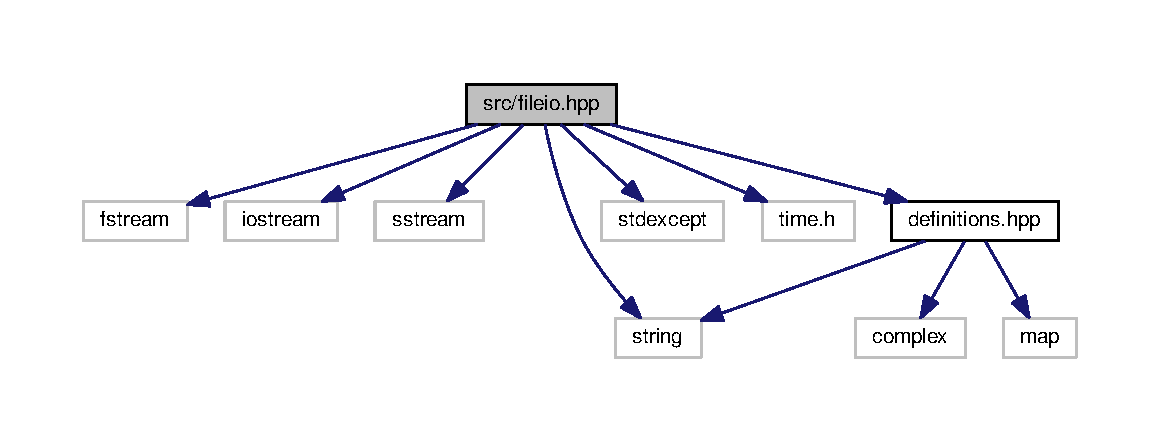
\includegraphics[width=350pt]{fileio_8hpp__incl}
\end{center}
\end{figure}
This graph shows which files directly or indirectly include this file\+:
\nopagebreak
\begin{figure}[H]
\begin{center}
\leavevmode
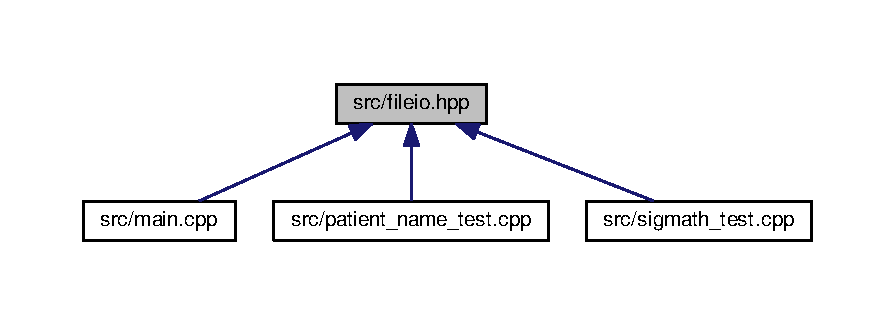
\includegraphics[width=350pt]{fileio_8hpp__dep__incl}
\end{center}
\end{figure}
\subsection*{Namespaces}
\begin{DoxyCompactItemize}
\item 
 \hyperlink{namespaceavda}{avda}
\end{DoxyCompactItemize}
\subsection*{Functions}
\begin{DoxyCompactItemize}
\item 
std\+::string \hyperlink{namespaceavda_ae20728e7e8ae50bf2f74849e538841ea}{avda\+::\+Patient\+Name} ()
\item 
std\+::map$<$ Side, \hyperlink{structDataParams}{Data\+Params} $>$ \hyperlink{namespaceavda_a46dc980b65ddfc24749ce25c1290e158}{avda\+::\+Read\+Params} (auto filename)
\item 
void \hyperlink{namespaceavda_aba04a08b41833ced32ec803d55a63bee}{avda\+::\+Write\+Params} (std\+::map$<$ Side, \hyperlink{structDataParams}{Data\+Params} $>$ my\+Map, auto filename)
\end{DoxyCompactItemize}
\subsection*{Variables}
\begin{DoxyCompactItemize}
\item 
const std\+::string \hyperlink{namespaceavda_ac568a0872c2c176d874b8b12f67f43ea}{avda\+::\+C\+S\+V\+\_\+\+H\+E\+A\+D\+E\+R} = \char`\"{}Time,Side,Frequency,Noise Level\char`\"{}
\item 
const std\+::string \hyperlink{namespaceavda_a8ee73ec0cb55d4a13e89949764dce89d}{avda\+::\+P\+A\+T\+I\+E\+N\+T\+\_\+\+P\+A\+T\+H} = \char`\"{}/home/pi/patients/\char`\"{}
\end{DoxyCompactItemize}


\subsection{Detailed Description}
contains functions related to the file I/\+O use in this program 

\begin{DoxyAuthor}{Author}
Samuel Andrew Wisner, \href{mailto:awisner94@gmail.com}{\tt awisner94@gmail.\+com} 

Nicholas K. Nolan 
\end{DoxyAuthor}
\begin{DoxyRefDesc}{Bug}
\item[\hyperlink{bug__bug000001}{Bug}]file is overly complicated and much more bug-\/prone \end{DoxyRefDesc}


Definition in file \hyperlink{fileio_8hpp_source}{fileio.\+hpp}.


\hypertarget{main_8cpp}{\section{src/main.cpp File Reference}
\label{main_8cpp}\index{src/main.\+cpp@{src/main.\+cpp}}
}
{\ttfamily \#include $<$array$>$}\\*
{\ttfamily \#include $<$cstdlib$>$}\\*
{\ttfamily \#include $<$iostream$>$}\\*
{\ttfamily \#include $<$map$>$}\\*
{\ttfamily \#include $<$pthread.\+h$>$}\\*
{\ttfamily \#include $<$string$>$}\\*
{\ttfamily \#include $<$unistd.\+h$>$}\\*
{\ttfamily \#include \char`\"{}definitions.\+hpp\char`\"{}}\\*
{\ttfamily \#include \char`\"{}fileio.\+hpp\char`\"{}}\\*
{\ttfamily \#include \char`\"{}process.\+hpp\char`\"{}}\\*
Include dependency graph for main.\+cpp\+:
\nopagebreak
\begin{figure}[H]
\begin{center}
\leavevmode
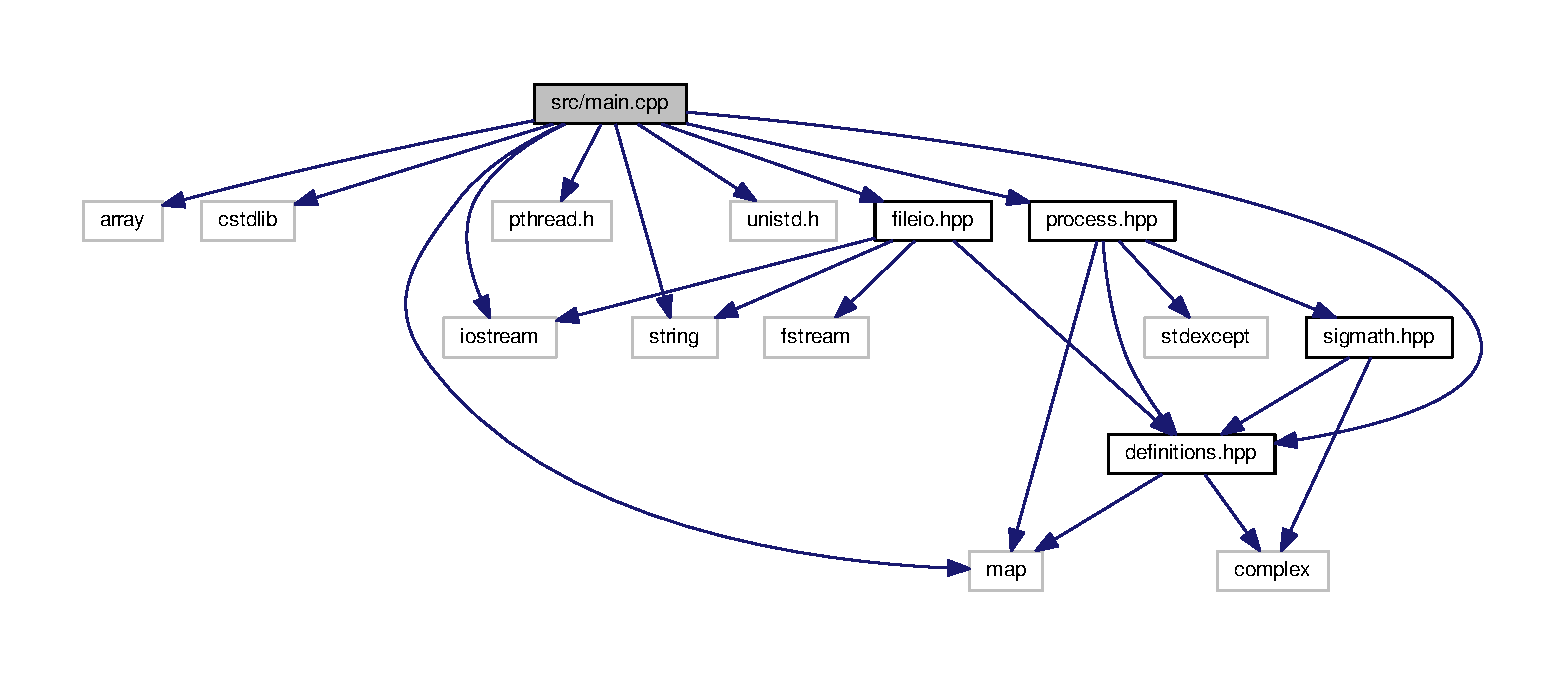
\includegraphics[width=350pt]{main_8cpp__incl}
\end{center}
\end{figure}
\subsection*{Functions}
\begin{DoxyCompactItemize}
\item 
int \hyperlink{main_8cpp_a3c04138a5bfe5d72780bb7e82a18e627}{main} (int argc, char $\ast$$\ast$argv)
\end{DoxyCompactItemize}


\subsection{Function Documentation}
\hypertarget{main_8cpp_a3c04138a5bfe5d72780bb7e82a18e627}{\index{main.\+cpp@{main.\+cpp}!main@{main}}
\index{main@{main}!main.\+cpp@{main.\+cpp}}
\subsubsection[{main}]{\setlength{\rightskip}{0pt plus 5cm}int main (
\begin{DoxyParamCaption}
\item[{int}]{argc, }
\item[{char $\ast$$\ast$}]{argv}
\end{DoxyParamCaption}
)}}\label{main_8cpp_a3c04138a5bfe5d72780bb7e82a18e627}
The main program for this progject. It will detect vasospasms over a period of days. 

Definition at line \hyperlink{main_8cpp_source_l00026}{26} of file \hyperlink{main_8cpp_source}{main.\+cpp}.



Here is the call graph for this function\+:
\nopagebreak
\begin{figure}[H]
\begin{center}
\leavevmode
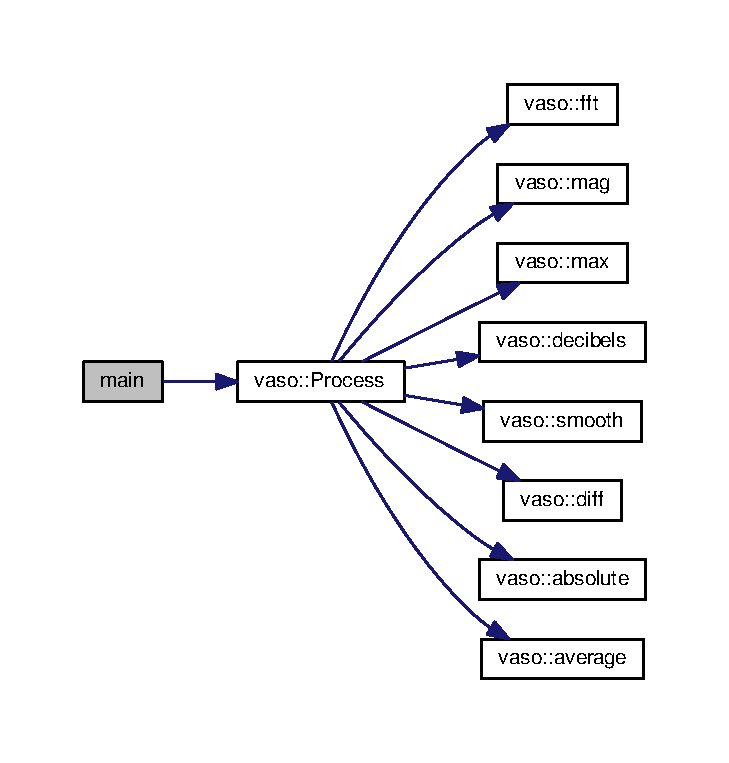
\includegraphics[width=350pt]{main_8cpp_a3c04138a5bfe5d72780bb7e82a18e627_cgraph}
\end{center}
\end{figure}



\hypertarget{sigmath_8hpp}{\section{src/sigmath.hpp File Reference}
\label{sigmath_8hpp}\index{src/sigmath.\+hpp@{src/sigmath.\+hpp}}
}
{\ttfamily \#include $<$complex$>$}\\*
{\ttfamily \#include \char`\"{}definitions.\+hpp\char`\"{}}\\*
Include dependency graph for sigmath.\+hpp\+:
\nopagebreak
\begin{figure}[H]
\begin{center}
\leavevmode
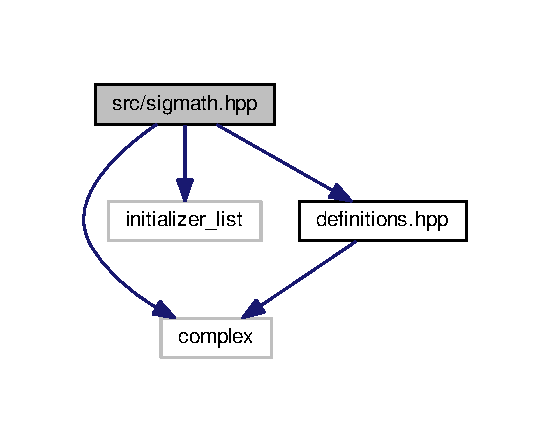
\includegraphics[width=197pt]{sigmath_8hpp__incl}
\end{center}
\end{figure}
This graph shows which files directly or indirectly include this file\+:
\nopagebreak
\begin{figure}[H]
\begin{center}
\leavevmode
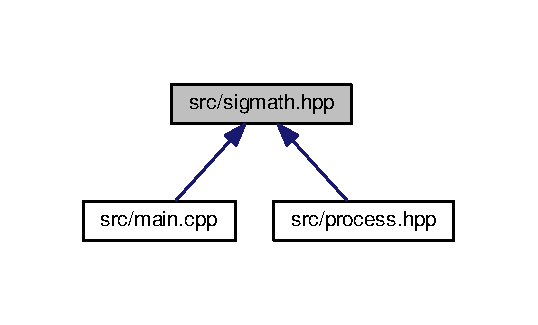
\includegraphics[width=258pt]{sigmath_8hpp__dep__incl}
\end{center}
\end{figure}
\subsection*{Namespaces}
\begin{DoxyCompactItemize}
\item 
 \hyperlink{namespacevaso}{vaso}
\begin{DoxyCompactList}\small\item\em contains functions related to the file I/\+O use in this program \end{DoxyCompactList}\end{DoxyCompactItemize}
\subsection*{Functions}
\begin{DoxyCompactItemize}
\item 
void \hyperlink{namespacevaso_a6ca90add966ce1773fc59a6883e6cd0c}{vaso\+::absolute} (\hyperlink{definitions_8hpp_aacdc525d6f7bddb3ae95d5c311bd06a1}{float32} $\ast$data, \hyperlink{definitions_8hpp_a1134b580f8da4de94ca6b1de4d37975e}{uint32} size)
\item 
\hyperlink{definitions_8hpp_aacdc525d6f7bddb3ae95d5c311bd06a1}{float32} \hyperlink{namespacevaso_ad3205136b1cd04b4c6b9d7be73661796}{vaso\+::average} (\hyperlink{definitions_8hpp_aacdc525d6f7bddb3ae95d5c311bd06a1}{float32} $\ast$data, \hyperlink{definitions_8hpp_a1134b580f8da4de94ca6b1de4d37975e}{uint32} size)
\item 
\hyperlink{structDataParams}{Data\+Params} \hyperlink{namespacevaso_a376413e791defec04a0faf329be1cbf4}{vaso\+::average} (\hyperlink{structDataParams}{Data\+Params} $\ast$params, \hyperlink{definitions_8hpp_adde6aaee8457bee49c2a92621fe22b79}{uint8} size)
\item 
void \hyperlink{namespacevaso_a9d0e5d69685ee494d286db6ece005156}{vaso\+::average} (\hyperlink{definitions_8hpp_aacdc525d6f7bddb3ae95d5c311bd06a1}{float32} $\ast$data, \hyperlink{definitions_8hpp_aacdc525d6f7bddb3ae95d5c311bd06a1}{float32} $\ast$avg, \hyperlink{definitions_8hpp_adde6aaee8457bee49c2a92621fe22b79}{uint8} count, \hyperlink{definitions_8hpp_a1134b580f8da4de94ca6b1de4d37975e}{uint32} size)
\item 
void \hyperlink{namespacevaso_af9bb2211cf3478333dfc1873bf316263}{vaso\+::decibels} (\hyperlink{definitions_8hpp_aacdc525d6f7bddb3ae95d5c311bd06a1}{float32} $\ast$data, \hyperlink{definitions_8hpp_a1134b580f8da4de94ca6b1de4d37975e}{uint32} size)
\item 
void \hyperlink{namespacevaso_a7d108bce812e906d8b1810815774c7ea}{vaso\+::diff} (\hyperlink{definitions_8hpp_aacdc525d6f7bddb3ae95d5c311bd06a1}{float32} $\ast$data, \hyperlink{definitions_8hpp_a1134b580f8da4de94ca6b1de4d37975e}{uint32} size)
\item 
void \hyperlink{namespacevaso_af74f08a8afd7967b6c2b3c2b0e5fb1e9}{vaso\+::fft} (\hyperlink{definitions_8hpp_a960be6b6614c08090c16574dba10a421}{cfloat32} $\ast$data, \hyperlink{definitions_8hpp_a1134b580f8da4de94ca6b1de4d37975e}{uint32} size)
\item 
void \hyperlink{namespacevaso_a5d355b5c326a852e2ce95c258450898c}{vaso\+::mag} (\hyperlink{definitions_8hpp_a960be6b6614c08090c16574dba10a421}{cfloat32} $\ast$orig, \hyperlink{definitions_8hpp_aacdc525d6f7bddb3ae95d5c311bd06a1}{float32} $\ast$newmags, \hyperlink{definitions_8hpp_a1134b580f8da4de94ca6b1de4d37975e}{uint32} size)
\item 
\hyperlink{structMaximum}{Maximum} \hyperlink{namespacevaso_a122846d728be312454a452d379915e10}{vaso\+::max} (\hyperlink{definitions_8hpp_aacdc525d6f7bddb3ae95d5c311bd06a1}{float32} $\ast$data, \hyperlink{definitions_8hpp_a1134b580f8da4de94ca6b1de4d37975e}{uint32} size)
\item 
void \hyperlink{namespacevaso_a5b7fc1a58199e2cac989f417a9faa1ce}{vaso\+::smooth} (\hyperlink{definitions_8hpp_aacdc525d6f7bddb3ae95d5c311bd06a1}{float32} $\ast$data, \hyperlink{definitions_8hpp_a1134b580f8da4de94ca6b1de4d37975e}{uint32} size, \hyperlink{definitions_8hpp_a05f6b0ae8f6a6e135b0e290c25fe0e4e}{uint16} order)
\end{DoxyCompactItemize}

\hypertarget{sound_8hpp}{\section{src/sound.hpp File Reference}
\label{sound_8hpp}\index{src/sound.\+hpp@{src/sound.\+hpp}}
}
{\ttfamily \#include $<$string$>$}\\*
{\ttfamily \#include \char`\"{}definitions.\+hpp\char`\"{}}\\*
Include dependency graph for sound.\+hpp\+:
\nopagebreak
\begin{figure}[H]
\begin{center}
\leavevmode
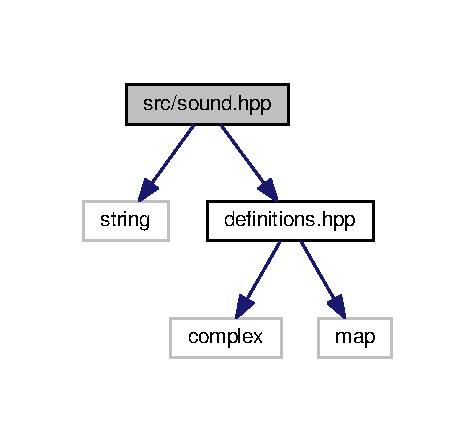
\includegraphics[width=220pt]{sound_8hpp__incl}
\end{center}
\end{figure}
\subsection*{Namespaces}
\begin{DoxyCompactItemize}
\item 
 \hyperlink{namespacevaso}{vaso}
\begin{DoxyCompactList}\small\item\em contains functions related to the file I/\+O use in this program \end{DoxyCompactList}\end{DoxyCompactItemize}
\subsection*{Functions}
\begin{DoxyCompactItemize}
\item 
void \hyperlink{namespacevaso_a7da499b9b1b5a492bea8ab8681e57c22}{vaso\+::play} (auto filename)
\end{DoxyCompactItemize}

\hypertarget{threadproc_8hpp}{\section{src/threadproc.hpp File Reference}
\label{threadproc_8hpp}\index{src/threadproc.\+hpp@{src/threadproc.\+hpp}}
}
{\ttfamily \#include $<$pthread.\+h$>$}\\*
{\ttfamily \#include \char`\"{}definitions.\+hpp\char`\"{}}\\*
Include dependency graph for threadproc.\+hpp\+:
\nopagebreak
\begin{figure}[H]
\begin{center}
\leavevmode
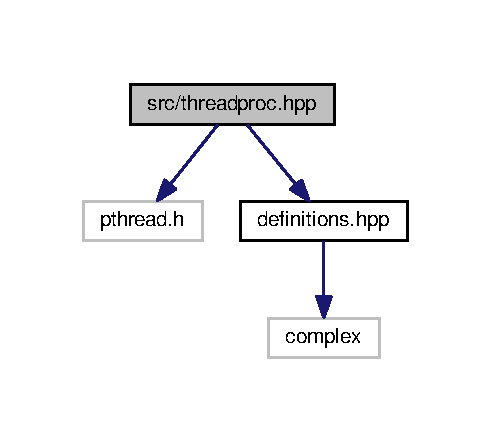
\includegraphics[width=236pt]{threadproc_8hpp__incl}
\end{center}
\end{figure}
This graph shows which files directly or indirectly include this file\+:
\nopagebreak
\begin{figure}[H]
\begin{center}
\leavevmode
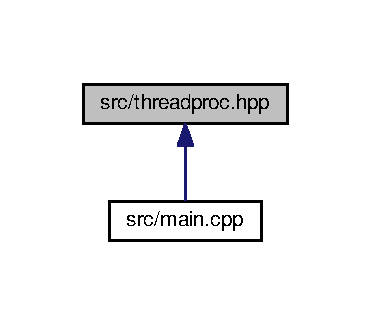
\includegraphics[width=178pt]{threadproc_8hpp__dep__incl}
\end{center}
\end{figure}
\subsection*{Namespaces}
\begin{DoxyCompactItemize}
\item 
 \hyperlink{namespacevaso}{vaso}
\begin{DoxyCompactList}\small\item\em contains functions related to the file I/\+O use in this program \end{DoxyCompactList}\end{DoxyCompactItemize}
\subsection*{Functions}
\begin{DoxyCompactItemize}
\item 
void $\ast$ \hyperlink{namespacevaso_a0579351ab19fb51460f6e9c50f234e22}{vaso\+::process} (void $\ast$procdata)
\item 
void \hyperlink{namespacevaso_aec526a2735f71ef68cea3e00ae943edf}{vaso\+::\+Start\+Processing} (\hyperlink{structProcData}{Proc\+Data} procdata)
\end{DoxyCompactItemize}

%--- End generated contents ---

% Index
\newpage
\phantomsection
\addcontentsline{toc}{chapter}{Index}
\printindex

\end{document}
